\scanpage{84}
\mspage{83}
\diagram{\begin{tikzcd}[ampersand replacement=\&]
H \handwritten{\arrow[r,dash,shift left=.7ex,draw=gray!45]} \handwritten{\arrow[r,"\handwritten{u_\nu}"]} \& G_{\handwritten{\nu}}\ \handwritten{(} \handwritten{\arrow[r]} \& G\handwritten{)}\ ,
\end{tikzcd}}
itself determined by knowledge of the homomorphism in the opposite direction on the character groups
\diagram{\begin{tikzcd}[ampersand replacement=\&]
Q \& \handwritten{\overline}{\handwritten{\underline}{Q}}^{\handwritten{*}} \handwritten{\arrow[l,"\handwritten{u_\nu^*}"']} \& \handwritten{\overline}{\handwritten{\underline}{Q}}^{\handwritten{*}} \handwritten{\arrow[l,"\handwritten{\lambda^\nu}"']} \handwritten{\arrow[ll,bend left=25,"\handwritten{|\lambda|}"']}\quad .
\end{tikzcd}}
We read from this diagram that, for the natural \rlap{h}isomorphism of the character group of $G_{\handwritten{\nu}}$ with $\rlap{$\phantom{Q}\unsure{\mathrm{Fr.}|\mathrm{Fl.}}$}\handwritten{\overline}{\handwritten{\underline}{Q}}^{\handwritten{*}}$, coming from the element $\handwritten{\underline}{f}_q\handwritten{\in}G_{\handwritten{\nu}}(\handwritten{\underline}{Q})$, \inserted{\handwritten{we}} \deleted{which gives}\inserted{\handwritten{have}}
\[
u_{\handwritten{\nu}}^{\handwritten{*}}(\handwritten{\lambda})=v_p(\handwritten{\lambda})/\handwritten{\nu}\quad .
\]
We thusx fin\rlap{e}d the following resul\rlap{(}t of Manin, stated in a prettier form and fre\rlap{a}ed of parasitic restrictive hypot\handwritten{h}eses:

\handwritten{\uline}{Proposition} 10.3. Let $(E,F_E)$ be an F-isocrystal over $\handwritten{\underline}{F}_q$, $q=p^{\handwritten{\nu}}$, and let us consider the cha\handwritten{\begin{tikzpicture}[baseline=0cm,x=1cm,y=1cm]\draw[thin] (0,0)..controls (.1,.02) and (.21,.15)..(.35,.24);\end{tikzpicture}}racteristic polynomial $f(T)$ of $F_E{}^{\handwritten{\nu}}$, \margin{\handwritten{NB if instead we take the valuation $\unsure{v_q|\nu_q}$ such that $v_q(q)=1$, we find the eigenvalues $v_q(\lambda_i)$ (without dividing by $\nu$)}}
let $\handwritten{\lambda}_1,..,\handwritten{\lambda}_N$ ($N=\operatorname{rang}E$) be its roots, and $c_1$ , $..,c_{\handwritten{N}}$ their normalized absolute values ($c_i=v_p(\handwritten{\lambda}_i)$, $v_p\mathopen{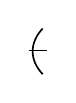
\begin{tikzpicture}[baseline=0cm,x=1cm,y=1cm]\draw[semithick] (.14,.45)..controls (-.03,.27) and (-.03,.05)..(.14,-.13);\draw[semithick] (-.04,.17)--(.2,.17);\end{tikzpicture}}p)=1$). Then \deleted{on} in $\operatorname{Rep}(\handwritten{\underline}{\unsure{\rlap{$G$}H|H|G}})\handwritten{\otimes}_{\handwritten{\underline}{Q}_p}\handwritten{\overline}{\handwritten{\underline}{Q}}_p\handwritten{\simeq}\operatorname{\unsure{\rlap{C}F|\rlap{E}F|E}criso}(\handwritten{\overline}{\handwritten{\underline}{F}}_q)\handwritten{\otimes}_{\handwritten{\underline}{Q}_p}\handwritten{\overline}{\handwritten{\underline}{Q}}_p$, the image of $(E,E_E)$ has as slopes the numbers $c_1/\handwritten{\nu}$, $...$ $c_N/\handwritten{\nu}$, \rlap{e}s\rlap{n}o that, if the \inserted{different}\handwritten{\begin{tikzpicture}[baseline=0cm,x=1cm,y=1cm]\draw[thin] (0,-.15)..controls (0,.1) and (.1,.2)..(.25,.2)--(2.7,.25)..controls (2.95,.26) and (3,.3)..(2.98,.4);\end{tikzpicture}} possible slopes are $\unsure{p_i|\deleted{p_i}}$\deleted{ with multiplicity} $p_i=s_i/r_i$ ($s_i,r_i\handwritten{\in}\handwritten{\underline}{Z}\deleted{r}$, $r_i\handwritten{\geq}1$, $(s_i,r_i)=1$) \rlap{\handwritten{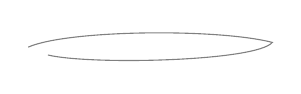
\begin{tikzpicture}[baseline=0cm,x=1cm,y=1cm]\draw[gray,thin] (0,.06)..controls (.5,.28) and (2.4,.3)..(3.1,.12)..controls (2.9,-.12) and (.8,-.17)..(.25,-.04);\end{tikzpicture}}}\deleted{\handwritten{$\unsure{d_ip_i\ \text{integer}|d_i,p_i\ \text{integers}|d_ip_i\in Q|d_ip_i\in Z}$}} with multiplicity $d_i$, we have $r_i\handwritten{\mid}d_i$ i.e\handwritten{,} $d_i=d'_ir_i$, and the image of $(E,F_E)$ in $\operatorname{Fcriso}(\handwritten{\overline}{\handwritten{\underline}{F}}_p)$ is isomorphic to $\handwritten{\sum_i}E_{p_i}^{d'_i}$.


\handwritten{\uline{Corollary}}
